% !Mode:: "Tex:UTF-8"
\chapter{细粒度的层次式贪婪地理路由}
\label{chap:6}
贪婪地理路由由于其简单性和低开销成为无线传感器网络中一种应用广泛的路由方法。但是固有的局部最小问题使得单纯的贪婪地理路由无法保证数据包的成功传输。为了克服局部最小问题,研究者提出了大量的解决方案。这些方法具有各自的优势和适用范围,在一定网络假设条件下实现了具有传输保证的路由协议。本章结合之前的各类方法的优势,提出了一种细粒度的层次式贪婪地理路由方法,称为FLYER(Fine-grainedLandmark-based greedY gEographic Routing)。FLYER不依赖于精确的节点位置信息,也不需要在每个节点中存储任何的全局状态信息,因此在实际的大规模无线传感器网络系统中具有良好的可用性和扩展性。另外,相对于之前的方法,FLYER在贪婪路由的成功率、路径失真率、负载均衡性等方面均具有一定的优势。本章从理论上证明了FLYER在满足一定的位置误差上限时具有传输保证,并通过大量的仿真实验验证了FLYER相对于之前方法的性能优势。
\section{引言}
路由协议是无线传感器网络中一种基本和关键的网络协议。贪婪地理路由作为一种很早就被提出的路由方式\upcite{routing_mobicom00},多年来一直得到了广泛的关注和研究\upcite{routing_wn,routing_podc03,routing_cc,routing_dialm2002,routing_mobihoc03}。贪婪地理路由协议使用节点的位置作为路由地址,每个节点以贪婪的方式将数据包发送至与目标距离最近的邻居节点。在密集和均匀部署的网络中,贪婪地理路由协议能够高效地运行,生成的路由路径非常接近最优路径(即最短路径)。但是,在稀疏或包含复杂形状空洞的网络中,贪婪地理路由往往频繁地遭遇局部最小,即当前节点由于没有与目标距离更近的邻居节点而导致贪婪路由失效。因此仅利用贪婪地理路由方法无法保证数据包的成功传输。

为了克服局部最小问题,研究者进行了大量的研究并提出了一系列的解决方案。这些方法在一定的网络假设条件下有效地解决了局部最小问题,并且具有各自的优势和适用性,但也都存在各自的局限性,如严格地依赖于精确的节点位置信息,需要保存全局的状态信息而导致扩展性较差,或者路由的性能较差,如路径的失真率较高、负载均衡性能较差等。例如,最早的GPSR(greedy perimeter stateless routing)\upcite{routing_mobicom00}方法假设节点的精确位置信息可知,提出了边缘路由策略,在出现局部最小时切换至边缘路由以恢复数据包的有效传输。但是在形状复杂的网络中,GPSR需要频繁地在贪婪路由和边缘路由之间切换,导致路径的失真率较高,即路径长度远远大于最短路径。另外,GPSR的负载均衡性较差,位于网络空洞边界上的节点被频繁地使用,导致其能量很快耗尽,而空洞变得越来越大。为了改善路由负载均衡性,Fang等人\upcite{routing_glider}提出了层次式路由方法,称为GLIDER。GLIDER方法首先从网络中选择少量的节点作为地标节点,将剩余的所有节点分配给距离最近的地标节点,从而将整个网络划分成一些类Voronoi分区。然后,GLIDER方法建立地标节点之间的全局路由表,并利用该路由表指导分区之间的路由决策。但是,传感器节点中严格受限的存储能力限制了全局路由表的大小,使得GLIDER方法的可扩展性较差。另外一类方法基于网络分割技术\upcite{shapesegmentation,segmentation_infocom09,segmentation_mobihoc10},其基本思想是按照一定的规则将网络通讯图分割为一系列具有良好形状的分区,在每个分区中贪婪路由能够保证始终有效。但是,将网络划分为可贪婪路由的分区是一项困难和复杂的工作,且节点中仍需要保存一定的全局分区信息。另外还有一些基于虚拟坐标的方法\upcite{planar_funke,virtual_coordinate_dialmpomc,virtual_coordinate_mobicom03,virtual_coordinate_infocom08,virtual_coordinate_infocom07,virtual_coordinate_ipsn09,virtual_coordinate_infocom10},其基本思想是利用图嵌入技术将网络图映射到一个虚拟坐标空间中,在该虚拟坐标空间中贪婪路由能够保证始终有效。这类方法不需要节点位置信息,也不需要在每个节点中保存全局的状态信息。但是,在坐标转换的过程中往往会产生较大的失真,使得路由路径的失真率无法得到保证。另外,Funke等人\upcite{routing_funke}提出了称为MGGR(macroscopic geographic greedy routing)的层次式贪婪地理路由协议,其基本思想是将地标路由和贪婪地理路由相结合,在地标网络层采用贪婪地理路由策略。MGGR不依赖精确的节点位置或全局路由表信息,且路径质量和负载均衡性均优于GPSR和GLIDER方法。但是,MGGR方法要求网络必须被分割成较大的分区才能保证得到的平面化地标网络图是连通的,而且平面化地标网络图比较稀疏,从而限制了方法生成的路由路径的质量。

近年来,随着无线传感器网络的规模越来越大,对路由协议的效率和可扩展性提出了更高的要求,贪婪路由由于其简单性成为一种优先的选择。但是,如何将贪婪地理路由有效地应用于大规模的实际网络,仍面临三个方面的主要挑战:第一,路由算法必须是存储高效的,即无须在每个节点中保存诸如路由表等全局状态信息;第二,路由算法必须对节点位置误差具有较好的鲁棒性,因为在实际的网络中获得所有节点的精确位置信息是不现实的,算法必须能够在一定的位置误差下有效地执行;第三,路由算法应该能够生成高质量的路由路径,如路径的失真率较低、路由的负载均衡性能较好。基于这三项具体的要求,之前的各类方法具有各自的优势,但是也都存在各自的局限性。

在大部分的实际网络中,贪婪路由过程中出现局部最小往往是少数现象,而大部分的贪婪传输是可以成功完成的。因此,为了克服少数的局部最小现象而采取一些全局的措施往往是代价过高和没有必要的,例如有些方法需要在所有的节点中保存诸如路由表等全局的状态信息,或者执行诸如虚拟坐标转换等全局的网络拓扑变换。这些措施往往导致贪婪路由丧失其原有的简单性的优势。本章结合之前的各类方法的优势,提出了一种细粒度的层次式贪婪地理路由方法,称为FLYER。FLYER的基本思想与MGGR类似,将贪婪地理路由和基于地标的路由相结合,在地标网络层执行贪婪地理路由。FLYER能够根据需要选择任意数量的地标节点,从而将网络中所有的节点划分成细粒度的Voronoi分区。另外,FLYER利用细粒度的平面化算法来构造具有良好连通性的平面化地标网络子图,并设计了灵活的平面化嵌入方法,以支持算法在出现局部最小时切换至边缘路由过程。网络中每个节点只需要保存自身所在分区以及平面化地标网络图中相邻分区中地标节点的坐标,以及自身到相邻分区的距离梯度信息(最短路径距离)。分区之间的(inter-tile)路由根据节点保存的地标节点的坐标信息以贪婪的方式完成,而分区内的(intra-tile)路由则根据节点保存的距离梯度信息贪婪地执行。FLYER在不依赖任何全局状态信息的情况下有效地克服了局部最小问题,并且在满足一定的节点位置误差上限时具有传输保证。本章从理论上证明了FLYER的正确性,并通过大量的仿真实验验证了方法的性能,实验结果显示FLYER在各项重要的性能指标上均优于之前的相关方法。

本章余下的部分组织如下:6.2节介绍本章采用的网络设置以及相关定义;6.3节介绍FLYER路由方法的具体设计,并给出必要的证明过程;6.4节通过大量的仿真实验评估方法的有效性和性能;最后6.5节对本章进行总结。
\section{问题描述}
本节阐述本章中采用的基本网络配置和假设,并介绍相关的术语和定义。

本章考虑部署在平面区域上的无线传感器网络,假设网络中每个节点有唯一ID。我们将网络通讯的连通关系图建模为一个简单无向图$G(V,E)$,其中点集$V$表示传感器节点,边集$E$表示节点之间直接的通讯链路。本章所设计的方法中需要利用已有的网络平面化算法\upcite{planar_tmc},该算法的理论证明是在Q-UDG图模型下完成,且要求参数为$\rho\ge1/\sqrt{2}$,因此本章也采用同样的假设。但实际上本章的设计并不依赖于特定的网络图模型。大量的仿真实验结果证明FLYER方法在一般的通图模型下仍然能够有效地运行并得到较好的结果。另外,本章假设网络中的每个节点都能够收集本节点所属分区以及平面化地标网络图中相邻分区的地标节点的坐标,以及自身到相邻的分区的距离梯度信息。这些信息可以简单地通过一次相邻分区之间的局部洪泛消息来实现,因此带来的通讯开销不会太高。

下面给出本章中涉及到的两个重要的概念,即路径失真率和节点位置的误差率,分别如定义\ref{def:601}和定义\ref{def:602}所述。
\begin{definition}\label{def:601}
给定网络$G$中任意的两个点$x,y$,设$P_G(x,y)$表示两点之间的一条路径,而$\|P_G(x,y)\|$表示路径的长度,则该路径的失真率定义为$\rho=\|P_G(x,y)\|/L_G(x,y)$,其中$L_G(x,y)$表示两点之间的最短路径长度。
\end{definition}

\begin{definition}\label{def:602}
节点位置的误差率$\delta$定义为可用的节点坐标$o$与实际的节点坐标$o^{'}$之间的欧式距离$|o, o^{'}|$与节点通讯半径$R_c$之间的比值,即$\delta=|o, o^{'}|/R_c$。
\end{definition}
另外,网络中节点位置误差率的上限限制了节点位置误差的范围,如误差率上限为0表示节点的位置是精确的,而误差率上限为1/2则表示已知的节点位置与实际的精确位置之间的欧式距离不超过$R_c/2$。
\begin{figure}[t]
  \centering
  \subfloat[网络连通图]{
    \label{fig:601a}
    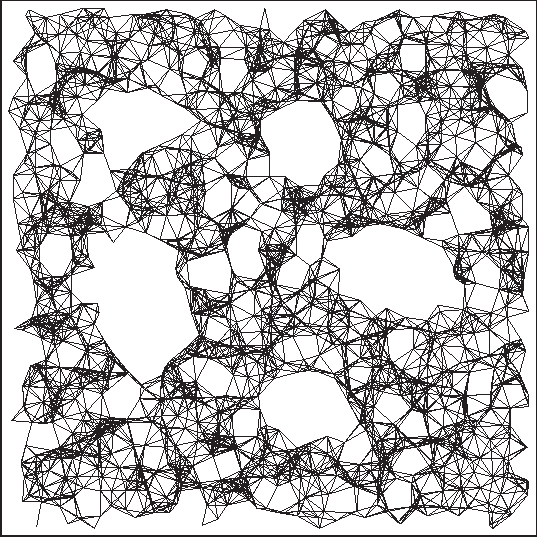
\includegraphics[width=.475\textwidth]{fig601-a}}\hspace{0.5em}%
  \subfloat[构建网络分区]{
    \label{fig:601b}
    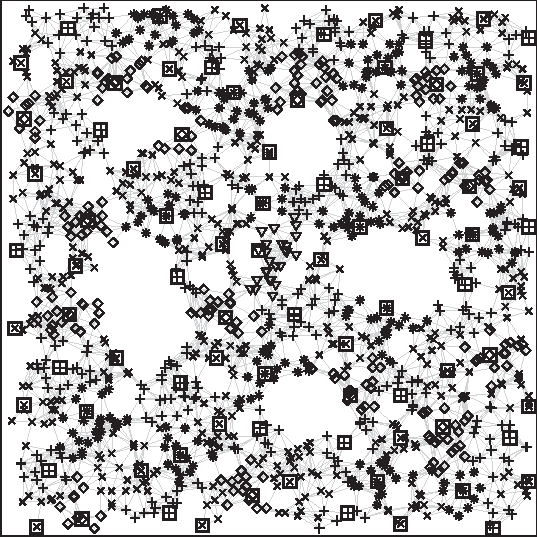
\includegraphics[width=.475\textwidth]{fig601-b}}\hspace{0.5em}%
  \subfloat[RWG图]{
    \label{fig:601c}
    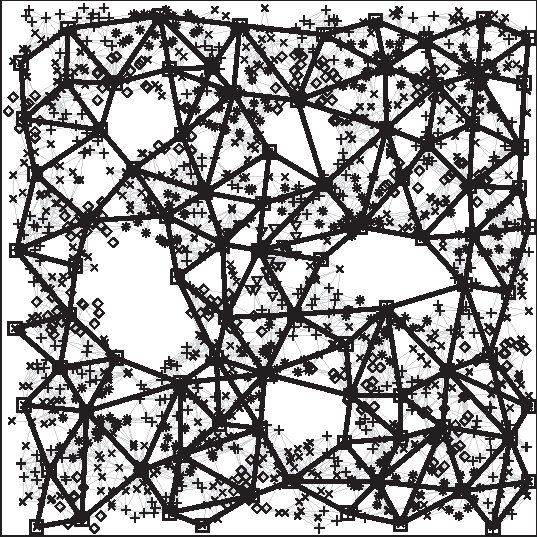
\includegraphics[width=.475\textwidth]{fig601-c}}\hspace{0.5em}%
  \subfloat[平面化地标网络图]{
    \label{fig:601d}
    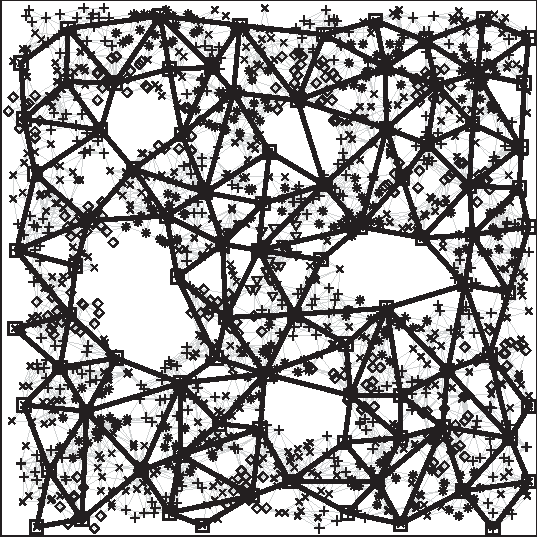
\includegraphics[width=.475\textwidth]{fig601-d}}
  \caption{FLYER方法中地标网络图的构建和平面化}
  \label{fig:601}
\end{figure}
\section{FLYER路由方法的设计}
本节介绍FLYER路由方法的具体设计,首先对方法的原理和主要过程进行概述,然后将方法分为几个主要的组件并分别进行具体的介绍。
\subsection{FLYER方法概述}
无线传感器网络不断增长的规模对路由协议的效率提出了严格的要求。贪婪路由由于其简单性得到了广泛的关注和应用。针对贪婪路由的局部最小问题,研究者提出了大量的解决方案。结合本章之前提出的三个主要的需求,我们对已有的各类方法的优势和适用范围进行了广泛的分析和比较。在此基础上,本章提出了FLYER路由方法。FLYER不依赖于精确的节点位置信息,不需要在每个节点中保存全局的状态信息,且能够生成高质量的路由路径。
\begin{figure}[h]
\centering
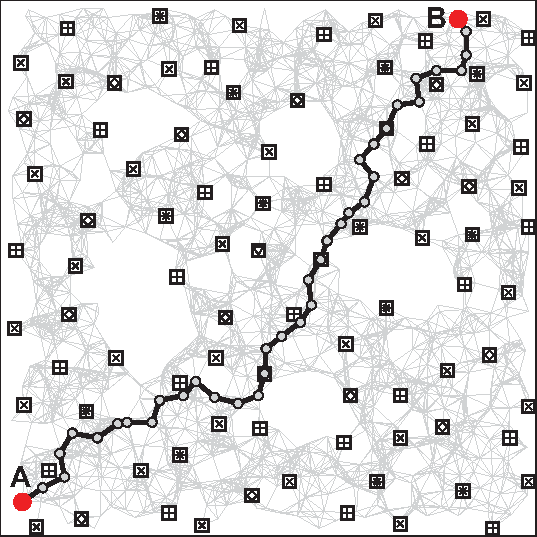
\includegraphics[width=0.5\textwidth]{fig602}
\caption{FLYER生成的路由路径的示例}
\label{fig:602}
\end{figure}

下面从方法的两个层面对FLYER的基本原理和主要过程进行概述。首先从网络中选出一个极大独立集作为地标节点,剩余的所有节点被分配给距离最近的地标节点,从而将整个网络划分为一系列基于地标节点的Voronoi分区。地标节点之间根据其所在分区的邻接关系建立边,从而构成了地标网络图。该地标网络图构成了FLYER方法的宏观层。例如,对于图\ref{fig:601a}所示的网络连通图,图\ref{fig:601b}表示网络分区划分的结果,而\ref{fig:601c}进一步地给出了构造出的地标网络图,其中小正方形表示地标节点,不同符号代表不同分区内的节点,粗线表示地标节点之间的边(同时构成了地标网络图中的边)。在地标网络图中,我们利用基于局部连通性信息的平面化算法抽取出一个平面化的地标网络子图,如图\ref{fig:601d}所示,并将该平面化子图嵌入在平面中。然后,FLYER就可以在地标网络图中执行贪婪路由,不同分区之间以地标节点的位置为地址,按照贪婪的方式传输数据。具体来讲,每个节点中记录着自身所在分区以及相邻分区的地标节点的坐标。数据包每进入一个新的分区,则根据节点中保存的坐标信息选择距离目标分区最近的相邻分区作为下一跳分区。当出现局部最小时,则切换至边缘路由方式,并利用抽取出的平面化子图及其平面嵌入来指导路由的决策。在微观层(即节点层),每个节点记录着自身到所有邻居分区的距离梯度信息(即到地标节点的最短路径的长度)。节点以贪婪的方式,将数据包发送至距离下一跳地标节点最近的邻居节点,从而完成了分区内的路由过程。分区之间和分区内的路由相结合,构成了FLYER的整个路由过程,保证了数据包从源节点发送至目标节点。图\ref{fig:602}给出了采用FLYER方法生成的节点$A$至节点$B$的一条路由路径,路径的长度为37跳,比较接近两点之间实际的最短路径(具体为34跳)。

下面通过将FLYER方法和MGGR方法\upcite{routing_funke}进行比较,直观地验证FLYER路由性能的优势。MGGR方法已经被证明比GPSR和GLIDER方法具有更优的性能,因此这里不再与这两种方法进行比较。总体来讲,FLYER方法比MGGR方法生成的路由路径的质量更高,例如路径失真率更低。这是因为FLYER方法比MGGR方法构造出的平面化地标网络图的连通性更好。图\ref{fig:603}给出的示例直观地验证了这一结果。图\ref{fig:603a}表示当网络分区直径为4时,MGGR得到的平面化地标网络图。可见,该平面化图分裂成多个连通分支。与之对比,图\ref{fig:601c}表示在同样的分区直径设置下,FLYER方法得到的平面化地标网络图。显然,FLYER方法得到的平面化地标网络图具有显著的连通性优势。另外,当网络分区直径增大时,FLYER方法始终具有明显的优势。例如,图\ref{fig:603b}和图\ref{fig:603c}分别给出了网络分区直径为10时,MGGR和FLYER方法得到的平面化地标网络图。显然,FLYER方法的结果仍然具有更好的连通性。由于更好的连通性代表着更多的路由选择,因此FLYER方法能够生成更高质量的路由路径。例如,图\ref{fig:604a}和图\ref{fig:604b}分别给出了在网络分区直径为10时,利用MGGR和FLYER方法得到的从点$A$至点$B$(最短路径长度为35)的路由路径,路径的长度分别为46和38。

接下来将FLYER划分为构建地标网络图、分区间路由、分区内路由三个组件,并分别对其设计进行具体的介绍。
\begin{figure}[t]
  \centering
  \subfloat[MGGR,分区直径为4]{
    \label{fig:603a}
    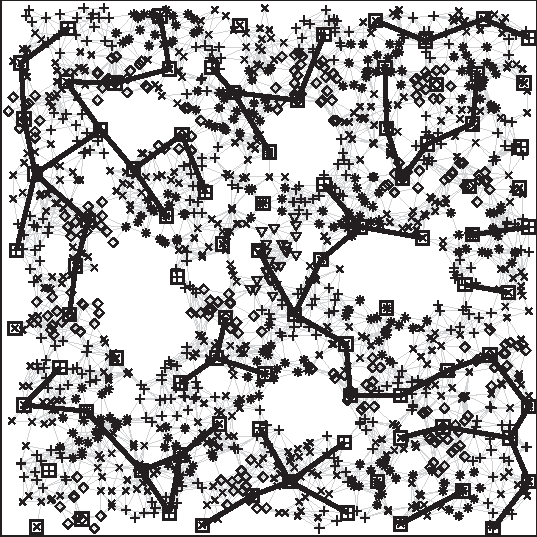
\includegraphics[width=.31\textwidth]{fig603-a}}\hspace{0.25em}
  \subfloat[MGGR,分区直径为10]{
    \label{fig:603b}
    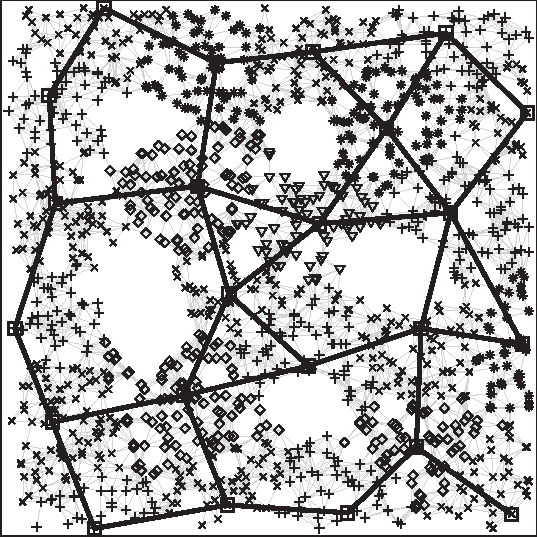
\includegraphics[width=.31\textwidth]{fig603-b}}\hspace{0.25em}
  \subfloat[FLYER,分区直径为10]{
    \label{fig:603c}
    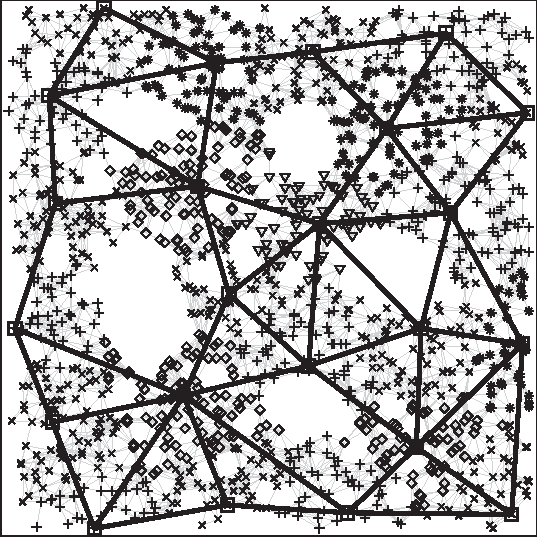
\includegraphics[width=.31\textwidth]{fig603-c}}
  \caption{FLYER与MGGR方法中平面化地标网络图的连通性的比较}
  \label{fig:603}
\end{figure}

\begin{figure}[h]
  \centering
  \subfloat[MGGR,分区直径为10]{
    \label{fig:604a}
    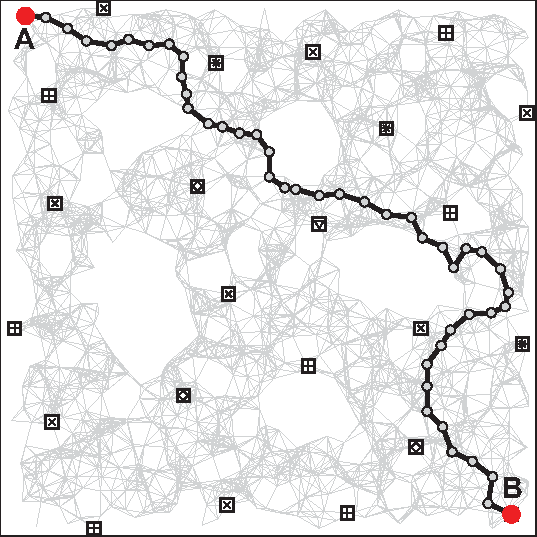
\includegraphics[width=.475\textwidth]{fig604-a}}\hspace{0.5em}
  \subfloat[FLYER,分区直径为10]{
    \label{fig:604b}
    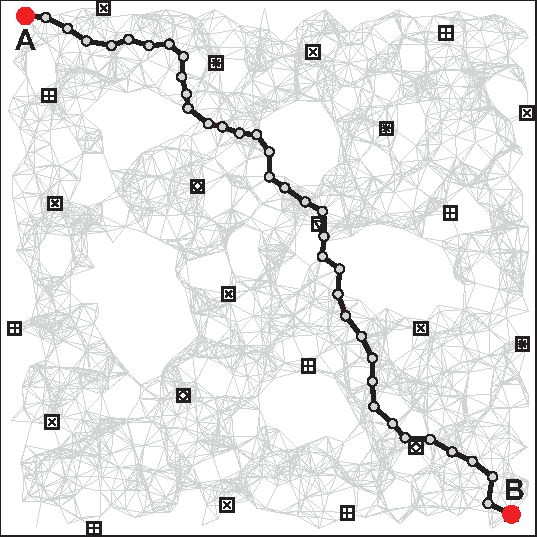
\includegraphics[width=.475\textwidth]{fig604-b}}
  \caption{FLYER与MGGR方法生成的路由路径的示例}
  \label{fig:604}
\end{figure}
\subsection{构建地标网络图}
该组件从网络中选择一组节点作为地标节点,并将整个网络划分为一系列基于地标节点的Voronoi分区。该过程主要是通过构造RWG图的方法来实现。RWG图的具体定义如第四章中定义4.2所述,这里不再赘述。

下面介绍RWG图的构建过程。首先,从网络中选择$k$跳极大独立集作为地标节点集。参数$k$的选择决定了网络分区的大小。为了实现细粒度的网络分区,$k$通常被设置为一个较小的常数(如$k$=2)。然后,剩余的所有节点被分配给距离自己最近的地标节点,如果节点拥有多个最近的地标节点则选择其中ID最大的。这样,整个网络就被划分为一系列以地标节点为标识的类Voronoi分区,如图\ref{fig:601b}所示为对图\ref{fig:601a}所示的网络连通图进行分区划分的结果。接下来按照如下的原则构造RWG图的边:对于任意的两个地标节点,如果它们所处的分区之间存在两个共享同一条边的节点,则在这两个地标节点之间连一条边,并作为RWG图中的边。至此,所有的地标节点和它们之间的边就构成了RWG图,确切地说是$(2k,1)$-RWG图,如图\ref{fig:601c}所示。这里需要强调的是,此时的RWG图并不一定是平面化的。另外,FLYER采用确定大小的分区设置,而不是GLIDER方法采用的大小不确定的分区。采用该方案的原因在于确定大小的分区提供了更好的负载均衡性能,包括计算开销、存储开销、路由负载等各个方面的负载都将分布更加均匀。

接下来对RWG图进行平面化处理。我们采用文献\upcite{planar_tmc}中提出的一种基于局部连通性信息的拓扑平面化算法TPS。TPS算法按照一定的原则对RWG图中的边进行修剪,最终得到一个平面化的RWG子图,表示为$RWG_{TPS}$。子图$RWG_{TPS}$的连通性和平面性都在理论上得到了证明。本章不详细介绍TPS算法的具体过程。图\ref{fig:601d}给出了平面化RWG子图的示例,可见该平面化图的分布较均匀,且具有良好的连通性。

平面化过程完成后,每个节点收集并存储自身所处分区以及在图$RWG_{TPS}$中相邻的所有分区的地标节点的坐标信息,以及本节点到所有相邻分区的地标节点的距离梯度信息(即最短路径长度)。在本章后面的内容中,若两个分区的地标节点之间在图$RWG_{TPS}$中存在一条边,则称这两个分区是相邻的。以上这些信息将被利用来指导分区间和分区内的路由过程,本章后面还将具体介绍。地标节点的坐标信息可以通过一个局部的洪泛消息获得。每个地标节点向自己的直接邻居发送一个包含自身坐标的洪泛消息,该洪泛消息仅在当前分区以及相邻分区内传播,因此传播范围的大小由分区的大小决定。由于地标节点的数量较少,且本章设计的方法采用了细粒度的分区划分,因此该洪泛消息的传播范围较小,引起的通讯开销不会太高。上述的距离梯度信息则可以通过每个地标节点构造局部的最短路径树获得,该过程同样可以通过之前的局部的洪泛消息来完成。因此,节点收集以上所需信息所引起的总的通讯开销不会太高。
\subsection{分区间路由}
平面化过程完成后,网络中所有的节点就可以在该平面化图的指导下执行路由过程。首先介绍分区间的路由策略,即从地标网络层的角度介绍数据包如何从源节点所处的分区被发送至目标节点所处的分区。

设$u$和$v$分别表示源节点和目标节点,$\tau(u)$和$\tau(v)$分别表示$u,v$所处的分区,$l(u)$和$l(v)$分别表示分区$\tau(u)$和$\tau(v)$的地标节点。假设源节点和目标节点位于不同的分区,即$\tau(u)\ne\tau(v)$。此时,节点$u$首先检查所有的相邻分区$\tau_1,\tau_2,...\tau_i$,分别计算它们的地标节点与目标地标节点(即目标节点所处分区的地标节点)之间的欧式距离,并选择距离最小的分区$\tau_j$作为下一跳分区。这一过程构成了FLYER的分区内路由过程。每个数据包重复执行该过程直至到达目标节点所在的分区。数据包在当前分区内的传递属于分区内路由的过程,将在下一节中介绍。

由于FLYER方法在地标网络层采用贪婪地理路由策略,则不可避免地面临局部最小问题,即当节点没有距离目标地标节点更近的相邻地标节点时,贪婪传输的过程将失败。为了解决这一问题,FLYER在出现局部最小时切换至边缘路由过程。边缘路由的思想与GPSR方法类似,区别在于FLYER是在宏观层(即地标网络层)执行边缘路由。当出现局部最小时,节点找出平面化图中所有的相邻地标节点,将该局部的平面化子图嵌入在平面上,然后按照一定的原则(如右手法则)选择下一跳地标节点。图\ref{fig:605}给出了利用右手法则执行边缘路由的简单示例,图中阴影部分表示网络空洞,黑点表示地标节点,实线表示$RWG_{TPS}$中的边,虚线表示当前分区的地标节点$S$到目标分区的地标节点$D$的方位角,虚线的长度即为局部最小距离。显然,$S$没有距离$D$更近的邻居地标节点,所以切换至边缘路由过程,并按照右手法则选择$X$作为下一跳地标节点。该过程重复地执行,直至出现到目标地标节点的距离小于局部最小距离的邻居,则切换回贪婪路由方式。
\begin{figure}[h]
\centering
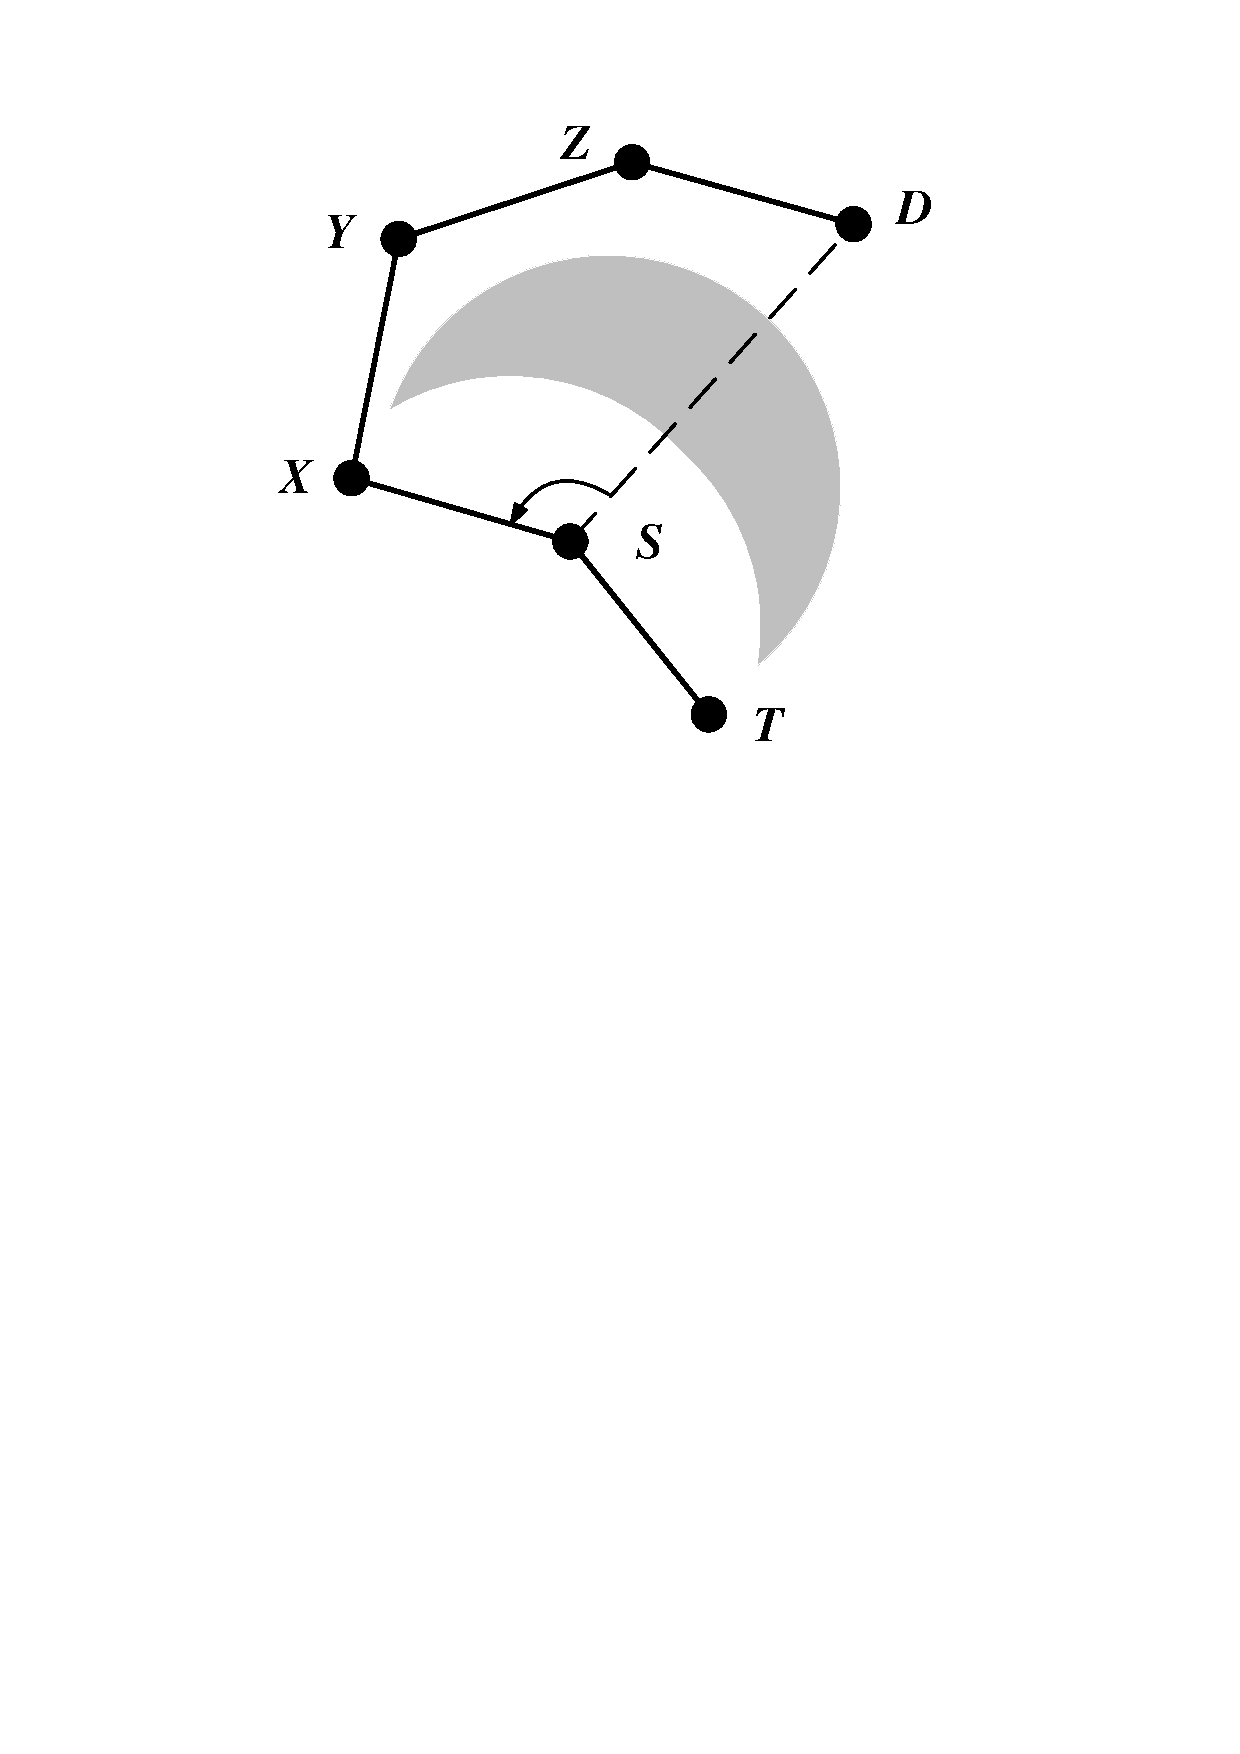
\includegraphics[width=0.4\textwidth]{fig605}
\caption{边缘路由和右手定则的原理示意图}
\label{fig:605}
\end{figure}

接下来介绍将局部平面化子图嵌入在平面中的过程。FLYER的嵌入过程不依赖精确的节点位置信息,并以完全分布式的方式来完成。设$\delta$为节点位置的误差率,$R_c$为节点的通讯半径,$a$为一个地标节点,$b$为$a$的一个相邻地标节点。我们首先按照如下的方式计算所有的相邻地标节点相对于$a$的方位角。假设以$b$为圆心画一个半径为$\delta*R$的圆,则$a$到该圆的两条切边构成了$b$相对于$a$的可视角,表示为$cone(a,b)$。如果$cone(a,b)$与$a$的其它所有的邻居地标节点的可视角均不重叠,则称$b$是$a$的一个有效邻居。如果$a$和$b$互为有效邻居,则称$(a,b)$是一条有效边。所有的地标节点和它们之间的有效边构成了$RWG_{TPS}$的平面化嵌入结果,并被利用来指导边缘路由过程。
\begin{figure}[h]
\centering
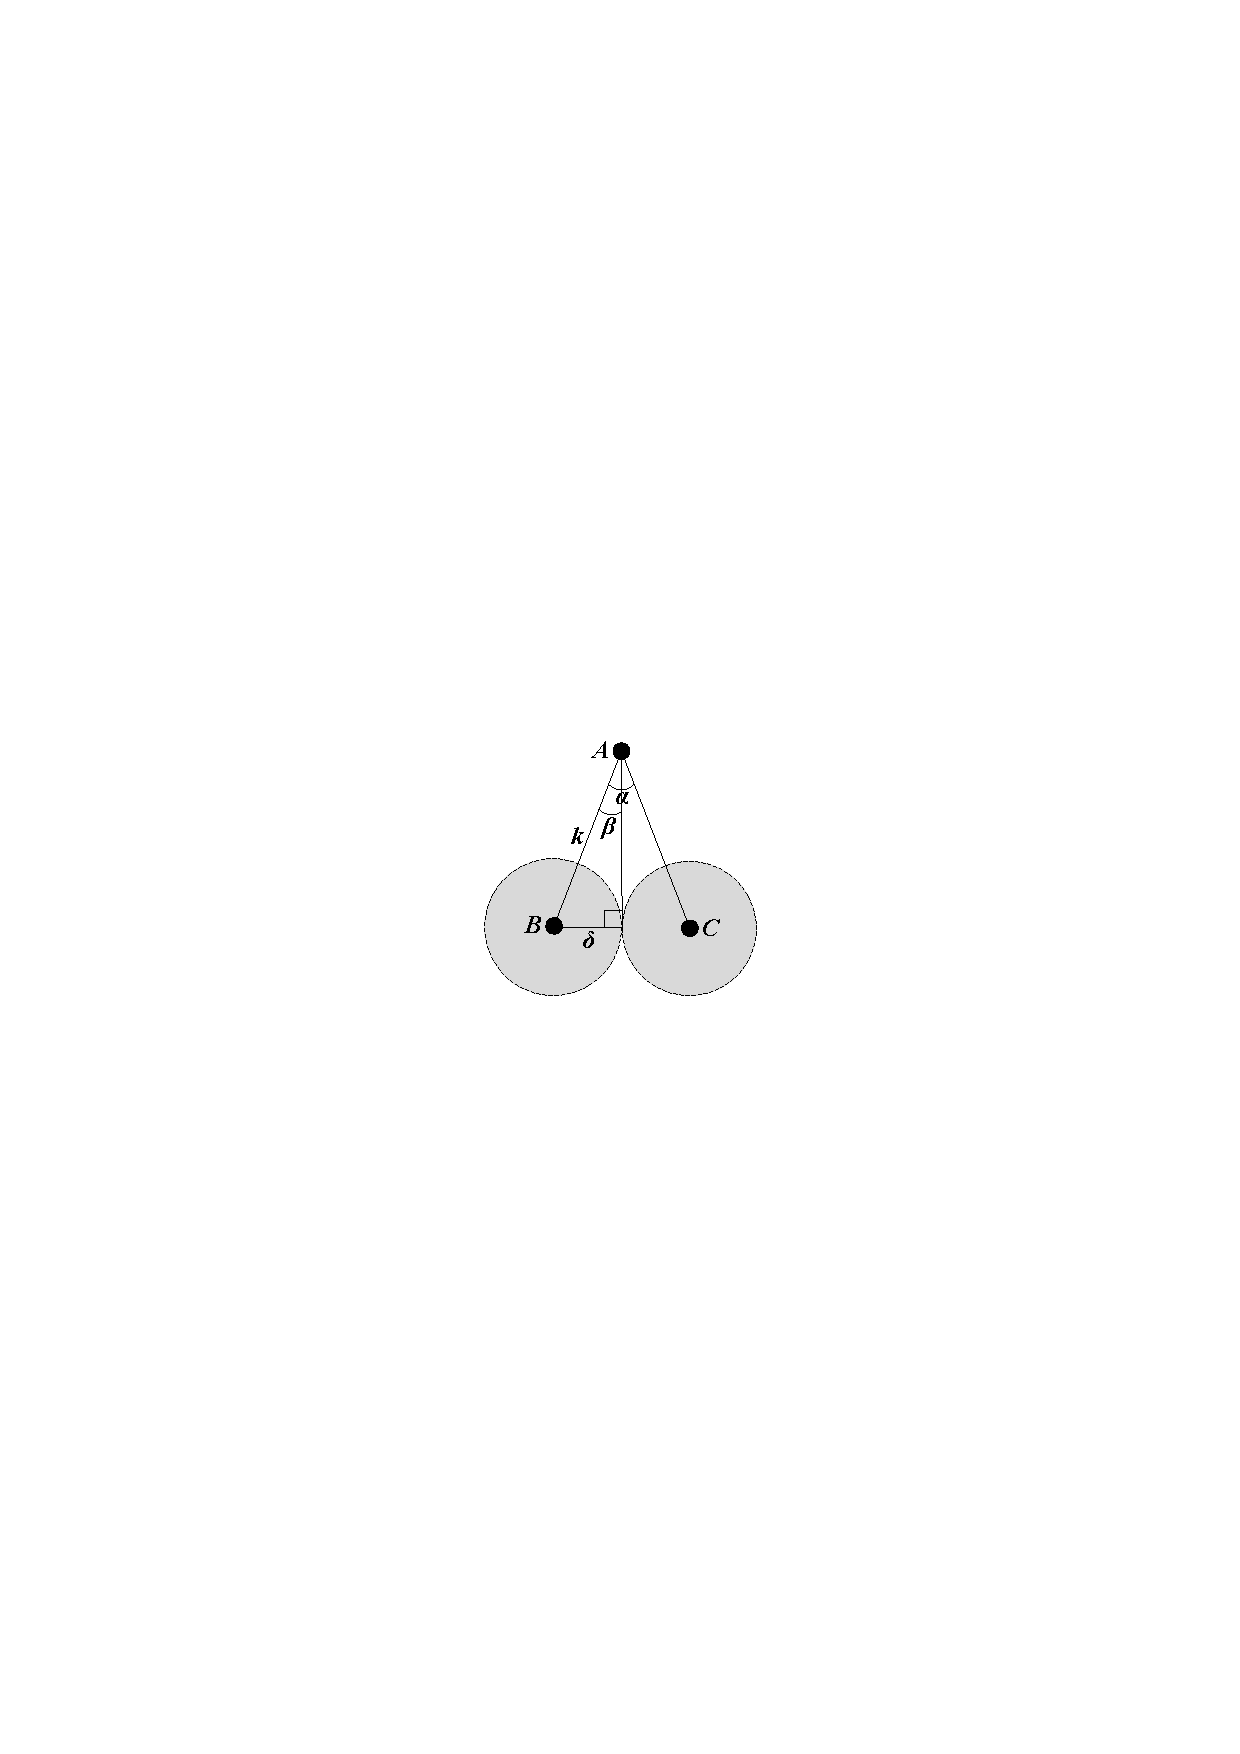
\includegraphics[width=0.35\textwidth]{fig605+}
\caption{节点位置误差率上限示意图}
\label{fig:605+}
\end{figure}

FLYER方法在一定的节点位置误差范围内可以保证数据包的成功传输。设地标节点为$k$跳独立集,平面化地标网络中地标节点度的最大值为$\Delta$,则定理\ref{theorem601}给出了具有传输保证的节点误差率的上限值。
\begin{theorem}
  \label{theorem601}
在节点位置的误差率不超过上限值$\delta=k\tan(\pi/\Delta)$时,FLYER方法具有传输保证。
\end{theorem}
\begin{proof}
为了证明FLYER方法具有传输保证,需要满足两个条件:(一)平面化地标网络图是连通的;(二)在误差率上限内,算法能够获得有效的平面化嵌入。

对于第一个条件,文献\upcite{planar_tmc}中已经进行了证明。下面证明第二个条件。首先考虑极限情况下可能的嵌入结果,如图\ref{fig:605+}所示,其中$A,B,C$ 表示三个地标节点,地标$A,B$之间的距离取最小值$k$(假设节点通讯半径为1)。角$\alpha$的最小度数为$\alpha=2\pi/\Delta$,由于地标节点$B,C$刚好成为$A$的有效邻居,则角$\beta=\alpha/2=\pi/\Delta$,由此我们可以得到$\delta=k\tan\beta=k\tan(\pi/\Delta)$。因此,有效嵌入的条件为$\delta\le{k\tan(\pi/\Delta)}$。 综上,在节点位置的误差率不超过上限值$\delta=k\tan(\pi/\Delta)$时,FLYER方法具有传输保证。
\end{proof}
\subsection{分区内路由}
本节分两种情况介绍分区内的路由策略。

第一种情况是数据包当前所处的分区不是目标分区,即目标节点不在当前分区内。在利用上述的分区间路由策略选定了下一跳分区后,我们需要将数据包从当前节点发送至下一跳分区。该过程通过利用节点中保存的到所有相邻地标节点的距离梯度信息来完成。具体来讲,每个节点以贪婪的方式将数据包发送至到下一跳地标节点的距离梯度值最小的邻居节点,直至数据包到达下一跳分区内的一个节点。由于该过程采用拓扑距离信息(即最小路径长度)作为贪婪路由的根据,因此不存在局部最小的情况。第二种情况是当前分区即为目标分区,则我们可以通过一个简单的分区内的洪泛消息将数据包发送至目标节点。由于FLYER采用了细粒度的分区设置,该洪泛消息的范围极小,因此该过程的通讯开销并不高。
\subsection{参数和开销分析}
本节分析FLYER中几个重要的参数及其对方法性能的影响,并对方法的各项开销进行分析。
\subsubsection{参数分析}
下面分析三个主要的参数及其对FLYER方法性能的影响,分别是分区大小、节点位置误差率,以及节点分布情况。

首先,分区大小是影响FLYER方法性能的关键参数,对贪婪路由成功率、路径失真率、负载均衡等各项性能均产生显著的影响。从直观上分析,较大的分区将更好地隐藏网络的细节拓扑特性,使得数据包更可能避免进入局部最小区域,因此将提供更高的贪婪路由成功率。分区大小对路径失真率的影响与网络中节点分布的情况密切相关。如果节点分布的随机性较强,或者网络中存在多个形状复杂的空洞,更大的分区设置将更好地避免出现局部最小现象,因此路径的长度更短,失真率较小。相反,如果网络分布较均匀,节点密度较高,且不存在空洞,则较大的分区设置将使得路由路径经历较多不必要的转弯,从而导致路径变长。在负载均衡性能方面,更大的分区设置将使路由路径更远离网络空洞的边界,从而提供更好的负载均衡性能。

然后分析节点位置误差的影响。从直观上分析,更大的节点误差率将导致路由的选择与实际的节点位置之间出现更大的偏差,因此导致贪婪传输的成功率降低。同时,路径出现偏差也将导致路径的长度增加,在误差达到一定程度时甚至将导致路由的失败。

最后分析节点分布情况对FLYER性能的影响,包括节点部署模型和网络密度两个方面。节点分布的随机性较强或者网络中存在大量空洞时,路由将经历更多的局部最小情况,并频繁地在贪婪路由和边缘路由之间切换,从而导致贪婪路由成功率较低,而路径的失真率较高。在这种情况下,可以通过选择较大的分区设置(如$k$=5)来改善路由性能。如果网络是均匀、密集部署的,则选择较小的分区设置将使路由更简单,而且输出更接近最短路径的路由路径。另外,在网络密度方面,由于FLYER方法主要工作在宏观的地标网络层,有效地避免了下层的节点密度对算法性能的影响,因此网络密度不会对算法的性能产生显著的影响。
\subsubsection{开销分析}
首先分析FLYER方法的时间复杂度。FLYER方法的时间复杂度主要来自平面化算法TPS的执行。按照文献\upcite{planar_tmc}中的分析,TPS算法的时间复杂度为$\mathcal{O}(\max\{\log\Delta\log^*n,\Delta^{k+2}\})$,其中$n$表示节点的数量,$k$表示在构造RWG图时选择的极大独立集的跳数,$\Delta$表示节点度的最大值。因此,当$\Delta$存在常数上限,而$k$为固定的常数时,这部分的时间复杂度降低为$\mathcal{O}(\log^*n)$。平面化地标网络图构造完成后,FLYER进入正常执行过程后的时间复杂度仅为常数复杂度$\mathcal{O}(1)$。

接下来分析FLYER方法的消息复杂度。FLYER方法的消息开销主要包括两部分,第一部分来自平面化算法,第二部分来自节点收据局部的位置和距离梯度信息的过程。同按照文献\upcite{planar_tmc}中的分析,平面化算法整体的消息复杂度为$\mathcal{O}(n)$,而具体到每个节点上则为常数复杂度$\mathcal{O}(1)$。在第二部分的开销中,每个节点只需要转发来自本节点所在分区的地标节点和相邻分区的地标节点的局部的洪泛消息,而每个节点的相邻地标节点的数量是存在常数上限的,所以具体到每个节点的消息开销为常数复杂度$\mathcal{O}(1)$。

最后分析FLYER方法的额外存储开销。在每个节点中,需要保存节点的所有相邻地标节点的坐标和距离梯度信息。由于相邻的地标节点的数量存在常数上限,而存储每个地标节点的相关信息需要的存储开销为常数,因此每个节点的整体存储开销为常数$\mathcal{O}(1)$。
\section{实验评估}
本节通过大量的仿真实验来评估FLYER方法在不同网络条件下的各项性能,并与之前的GPSR\upcite{routing_mobicom00}和MGGR\upcite{routing_funke}方法进行比较。
\begin{figure}[t]
\centering
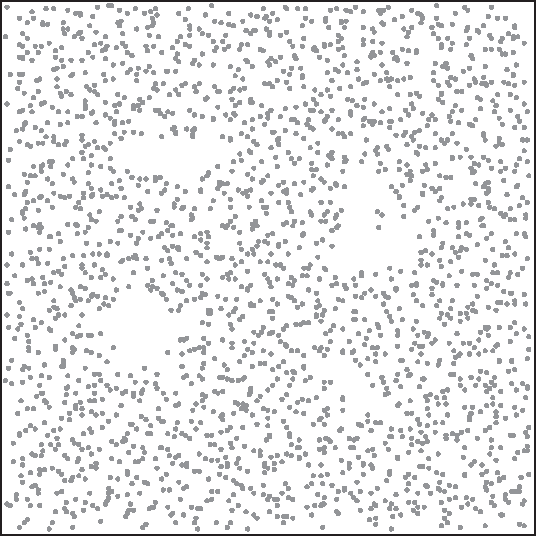
\includegraphics[width=0.4\textwidth]{fig606}
\caption{贪婪路由成功率评估实验中使用的网络}
\label{fig:606}
\end{figure}
\subsection{实验设置}
实验将对FLYER方法的多个性能指标进行全面的评估,如贪婪路由成功率、路径失真率、负载均衡性、存储开销等,并对一些关键的参数及其对方法性能的影响进行分析,如节点位置误差率、节点通讯模型、分区大小设置等。仿真实验中所采用的网络部署的随机性较强,从而充分地验证了方法的鲁棒性。另外,仿真实验中采用了多种不同形状的网络,并在网络中设置了多种不同形状和大小的网络空洞,而FLYER方法始终能得到稳定的结果。由于篇幅的限制,本节仅给出了一些具有代表性的网络实例,而省略了其它一些相似的实验过程和结果。
\subsection{贪婪路由成功率}
首先评估FLYER方法在不同网络设置下仅使用贪婪路由策略时的传输成功率,并与GPSR和MGGR方法进行比较。
\begin{figure}[t]
  \centering
  \subfloat[UDG模型下的贪婪路由成功率]{
    \label{fig:607a}
    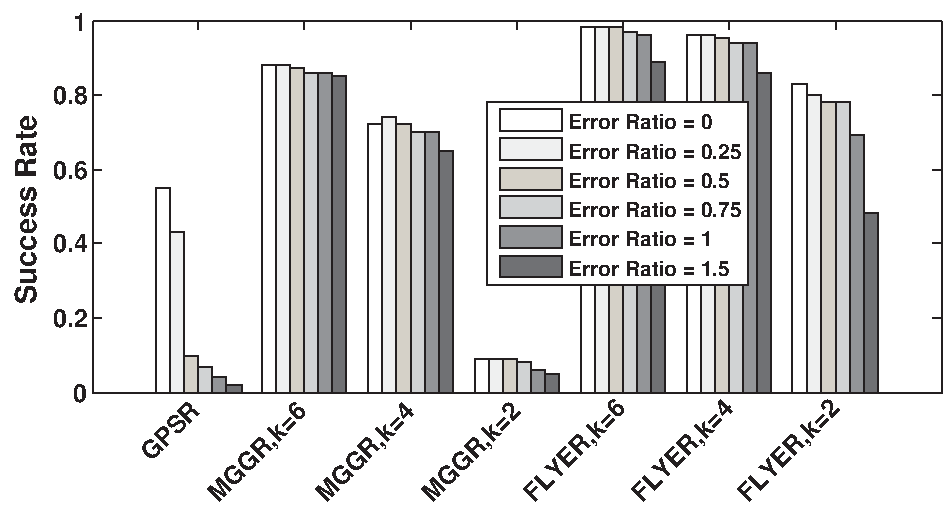
\includegraphics[width=.8\textwidth]{fig607-a}}\hspace{2em}
  \subfloat[Q-UDG模型下的贪婪路由成功率]{
    \label{fig:607b}
    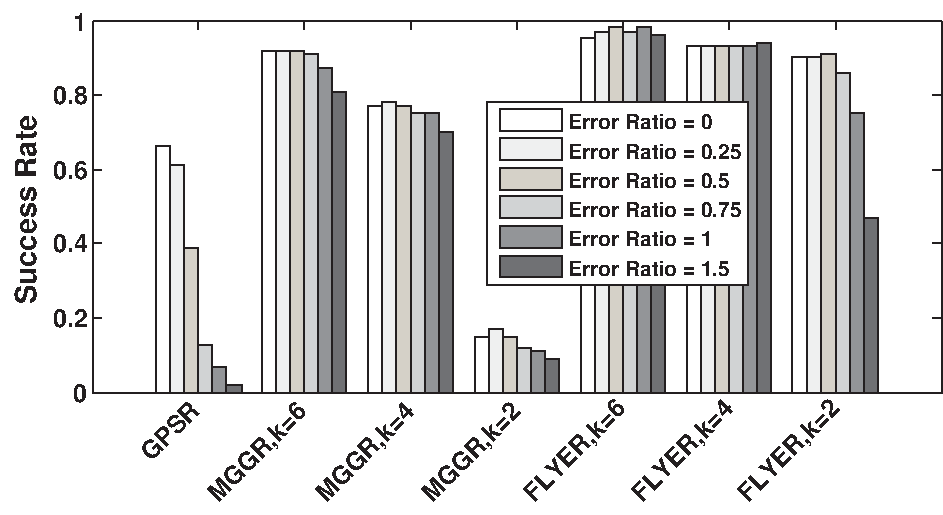
\includegraphics[width=.8\textwidth]{fig607-b}}
  \caption{贪婪路由成功率的评测结果}
  \label{fig:607}
\end{figure}

实验采用的网络连通图如图\ref{fig:606}所示,2308个节点随机地部署在正方形区域内,网络中包含多个空洞。我们随机地从网络中选择1000个节点对,计算它们之间在不同的节点位置误差下的贪婪路由成功率。图\ref{fig:607a}和图\ref{fig:607b}分别给出了三种方法在UDG和0.75-Q-UDG模型下的评测结果,其中$x$轴表示不同的方法,$y$轴表示贪婪路由成功率。从图\ref{fig:607}所示的结果中,我们可以得到如下几个重要的结论。

第一,在同样的网络条件和参数设置下,FLYER方法的贪婪路由成功率始终高于GPSR和MGGR方法。下面对其原因进行分析。相对于GPSR方法,FLYER有效地利用了地标路由的优势。具体来讲,FLYER方法运行在宏观的地标网络层,较好地隐藏了网络中的细节特征,如较小的网络空洞,因此避免了大部分的局部最小现象,使得贪婪路由的成功率显著提高。而相对于MGGR方法,FLYER方法提供了具有更好连通性的平面化地标网络,从而为贪婪路由提供了更多的选择,贪婪路由的成功率也相应得到改善。特别是在网络分区设置较小时,FLYER相对于MGGR方法的优势更明显。在$k$=2(即分区直径为4)时,MGGR的贪婪路由成功率甚至低于GPSR。

第二,FLYER方法对节点位置的误差具有更好的鲁棒性。具体来讲,GPSR方法的贪婪路由成功率随着节点误差率的增加而快速地降低。这是因为GPSR运行在初始网络中,节点位置的误差将使得贪婪地理路由的选择出现较大的偏差,贪婪传输的成功率随之降低。FLYER方法和MGGR方法的成功率随着位置误差率的增加而缓慢地降低。这是因为地标路由运行在宏观层,有效地缓解了底层的节点位置偏差对路由性能的影响。在误差率为1.5时,两种方法的贪婪路由成功率依然是比较高的。另外需要强调的是,在相同的误差率下,FLYER方法的成功率始终高于MGGR方法。
\begin{figure}[t]
\centering
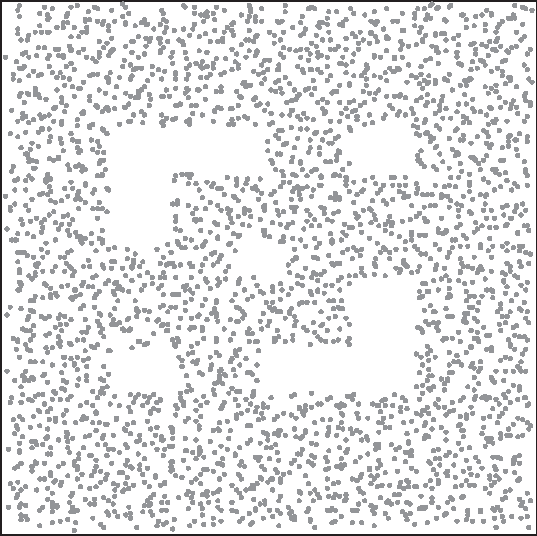
\includegraphics[width=0.4\textwidth]{fig608}
\caption{路径失真率评估实验中使用的网络}
\label{fig:608}
\end{figure}

第三,FLYER方法对分区大小具有更好的鲁棒性。MGGR方法的贪婪路由成功率随着分区的减小而快速地降低。这是因为在较小的分区设置下,MGGR提取的平面化地标网络图的连通性较差,从而导致贪婪路由频繁地失败。FLYER方法的贪婪路由成功率随着分区的减小而缓慢地降低,但是相对于MGGR方法,FLYER方法对分区大小的鲁棒性有了显著的改善。另外,在相同的分区设置下,FLYER方法的成功率始终高于MGGR方法。

第四,FLYER方法在UDG模型和Q-UDG模型下的贪婪路由成功率没有明显的差别,从而充分地证明了FLYER方法对通讯图模型的鲁棒性。
\subsection{路径失真率}
接下来评估FLYER方法在不同的网络设置下的路径失真率,并与GPSR和MGGR方法进行比较。
\begin{figure}[t]
  \centering
  \subfloat[UDG模型下的路径失真率]{
    \label{fig:609a}
    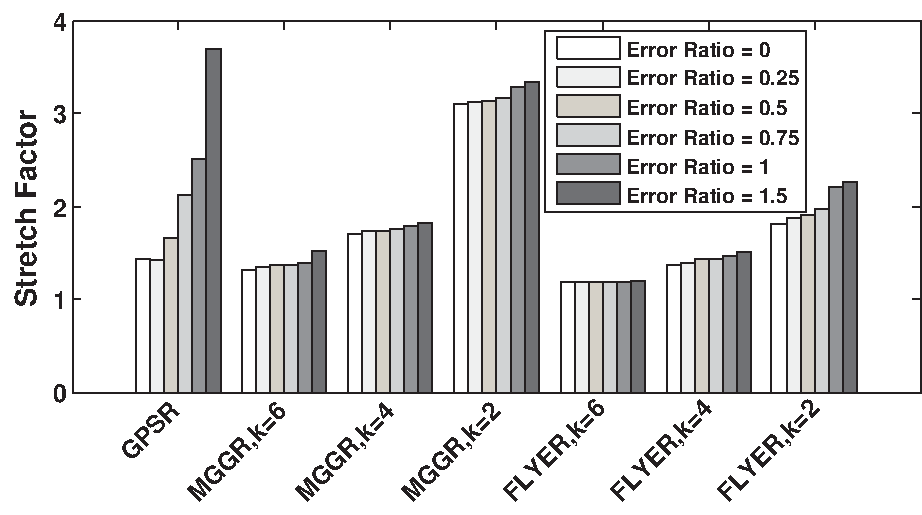
\includegraphics[width=.8\textwidth]{fig609-a}}\hspace{2em}
  \subfloat[Q-UDG模型下的路径失真率]{
    \label{fig:609b}
    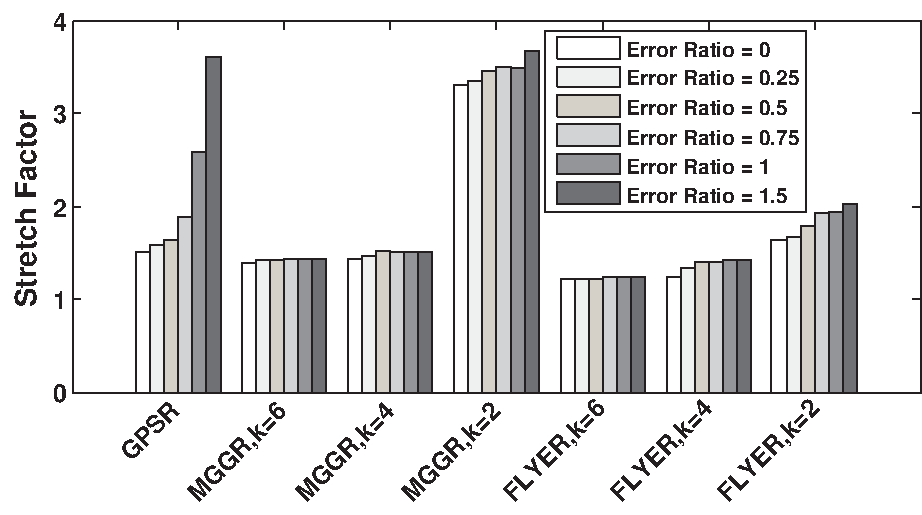
\includegraphics[width=.8\textwidth]{fig609-b}}
  \caption{路径失真率的评测结果}
  \label{fig:609}
\end{figure}

实验采用的网络连通图如图\ref{fig:608}所示,3128个节点部署在正方形区域内,网络中包含多个空洞。我们仍然随机地从网络中选择1000个节点对,计算它们之间的路径在不同的节点位置误差下的失真率。图\ref{fig:609a}和图\ref{fig:609b}分别给出了三种方法在UDG和0.75-Q-UDG模型下的评测结果,其中$x$轴表示不同的方法,$y$轴表示路径失真率。从图\ref{fig:609}所示的结果中,我们可以得到如下几个重要的结论。

第一,在同样的网络条件和参数设置下,FLYER方法的路径失真率始终低于GPSR和MGGR方法。下面对其原因进行分析。相对于GPSR方法,FLYER方法采用了层次式的地标路由策略,因此避免了复杂网络中大部分的局部最小现象,产生的路径的长度更接近最短路径。而相对于MGGR方法,FLYER方法提取出的平面化地标网络图具有更好的连通性,因此在路由决策时的可选择性更广,产生的路径也能够变得更短。第二,FLYER方法在路径失真率方面,依然表现出对节点位置误差的良好的鲁棒性。这同样是因为FLYER的层次式路由缓解了底层节点位置误差对上层路由性能的影响。第三,路径失真率随着分区大小的增加而增加。由于实验采用的网络中包含多个空洞,在原始网络中执行贪婪路由时将遭遇较多的局部最小现象。较大的分区设置将更好地避免数据包进入局部最小区域,因此产生的路径将更平滑且更短。在路径失真率方面,FLYER 方法提供了比MGGR方法更好的对分区大小的鲁棒性,其原因依然源于FLYER方法得到的平面化地标网络图具有更好的连通性。第四,FLYER方法的路径失真率仍然与通讯图模型没有明显的关系,从而再次证明了FLYER方法对通讯图模型的良好鲁棒性。
\begin{figure}[t]
\centering
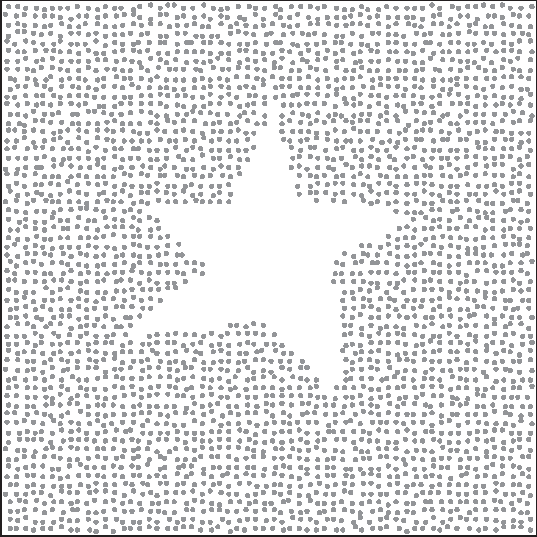
\includegraphics[width=0.4\textwidth]{fig610}
\caption{负载均衡性评估实验中使用的网络}
\label{fig:610}
\end{figure}
\subsection{负载均衡性}
下面对FLYER方法的负载均衡性进行评估,并与之前的GPSR和MGGR方法进行比较。

实验采用的网络连通图如图\ref{fig:610}所示,3237个节点部署在包含空洞的正方形区域内,平均节点度为10。我们仍然随机地从网络中选择1000个节点对并利用不同的路由方法得到它们之间的路由路径。然后,对于不同的方法,我们分别计算每个节点在所有的路径中出现的次数,并用可视化的方法表示出来,如图\ref{fig:611}所示,其中点的颜色越深表示对应节点的路由负载越高。
\begin{figure}[t]
  \centering
  \subfloat[GPSR]{
    \label{fig:611a}
    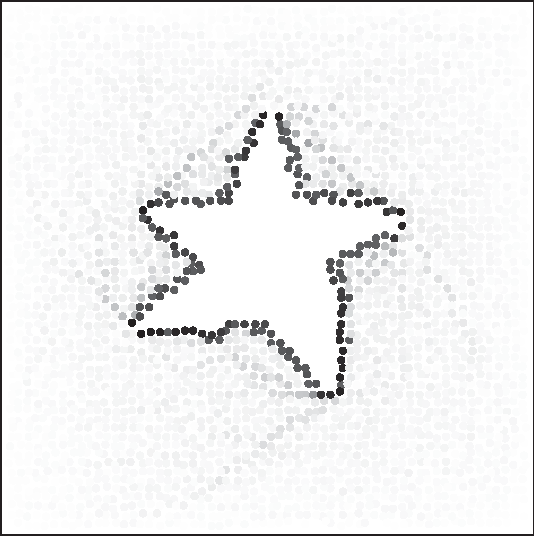
\includegraphics[width=.475\textwidth]{fig611-a}}\hspace{0.5em}%
  \subfloat[FLYER,$k$=3]{
    \label{fig:611b}
    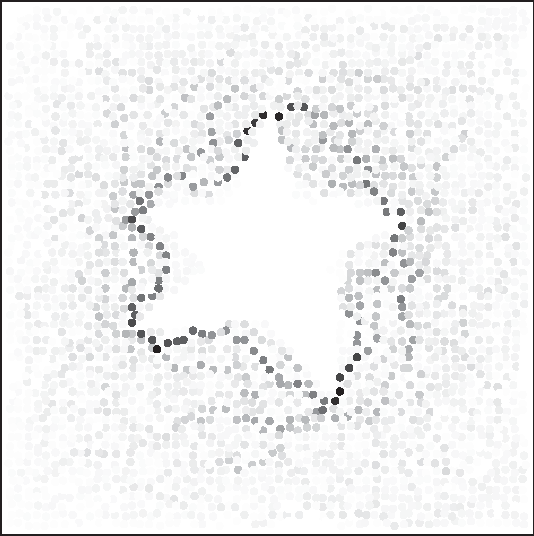
\includegraphics[width=.475\textwidth]{fig611-b}}\hspace{0.5em}%
  \subfloat[FLYER,$k$=5]{
    \label{fig:611c}
    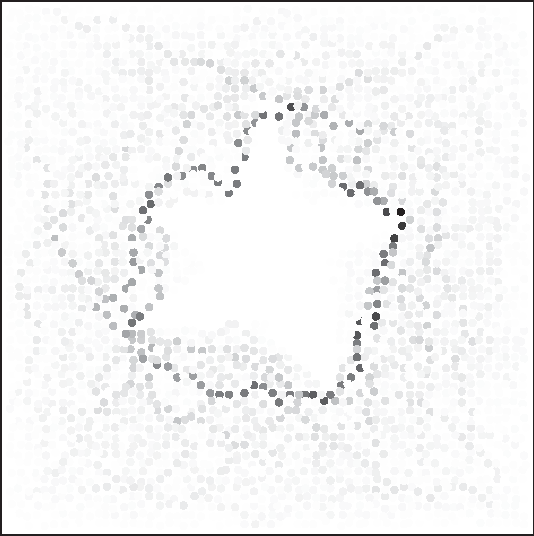
\includegraphics[width=.475\textwidth]{fig611-c}}\hspace{0.5em}%
  \subfloat[MGGR,$k$=5]{
    \label{fig:611d}
    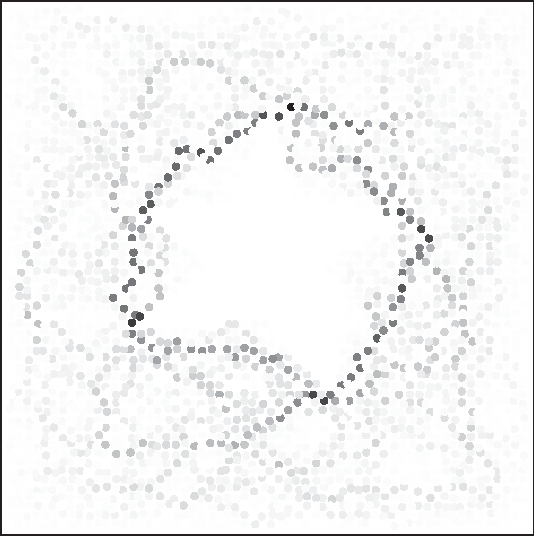
\includegraphics[width=.475\textwidth]{fig611-d}}
  \caption{负载均衡性的评测结果}
  \label{fig:611}
\end{figure}

从实验结果可以看出,GPSR方法的负载均衡性能最差,如图\ref{fig:611a}所示。位于空洞边界上的节点的负载非常高,这将导致这些节点的能量很快被耗尽,而空洞也将变得越来越大。FLYER方法有效地改善了负载均衡性能,如图\ref{fig:611b}-\ref{fig:611c}所示分别为$k$=3和$k$=5时FLYER的路由负载分布情况。这是由于FLYER采用的基于分区的路由策略使得数据包在到达空洞边界之前,就被均匀地分散至位于空洞附近的分区内的节点上。另外,较大的网络分区设置往往使得数据包更加远离空洞边界,从而进一步地改善路由负载均衡性能。但是,过大的分区设置将不再对负载均衡性能的改善发挥明显的作用,反而将导致失去基于分区路由的优势。根据我们的仿真实验,一般情况下可以将$k$=5作为分区大小的上限。在负载均衡性能方面,MGGR方法与FLYER方法没有显著的区别,如图\ref{fig:611d}给出了$k$=5时MGGR方法的路由负载的分布情况。
\subsection{存储开销}
最后对FLYER方法的存储开销进行评估。
\begin{table}[h]
\caption{FLYER路由方法的存储开销}
\label{table601}
\centering
\begin{tabular}[width=0.75\textwidth]{ccccc}
\toprule[1.5pt]
{\hei 节点数量} & {\hei 平均节点度} & {\hei $k$} & {\hei 地标节点数量} & {\hei 存储开销(bytes)}\\\midrule[1pt]
\multirow{6}{*}{1440} & \multirow{2}{*} {5.20}  & 2 & 4.76 & 23.78 \\
                      %\cline{3-5}
                      &                         & 5 & 4.68 & 23.38 \\
                      %\cline{2-5}
                      & \multirow{2}{*} {11.12} & 2 & 5.01 & 25.04 \\
                      %\cline{3-5}
                      &                         & 5 & 4.04 & 20.20 \\
                      %\cline{2-5}
                      & \multirow{2}{*} {17.15} & 2 & 4.90 & 24.51 \\
                      %\cline{3-5}
                      &                         & 5 & 3.96 & 19.79 \\\midrule[1pt]
\multirow{6}{*}{2246} & \multirow{2}{*} {5.20}  & 2 & 4.83 & 24.16 \\
                      %\cline{3-5}
                      &                         & 5 & 4.83 & 24.13 \\
                      %\cline{2-5}
                      & \multirow{2}{*} {11.12} & 2 & 5.31 & 26.57 \\
                      %\cline{3-5}
                      &                         & 5 & 4.67 & 23.35 \\
                      %\cline{2-5}
                      & \multirow{2}{*} {17.15} & 2 & 5.11 & 25.57 \\
                      %\cline{3-5}
                      &                         & 5 & 3.85 & 19.24 \\\midrule[1pt]
\multirow{6}{*}{3245} & \multirow{2}{*} {5.20}  & 2 & 4.83 & 24.15 \\
                      %\cline{3-5}
                      &                         & 5 & 4.77 & 23.83 \\
                      %\cline{2-5}
                      & \multirow{2}{*} {11.12} & 2 & 5.44 & 27.21 \\
                      %\cline{3-5}
                      &                         & 5 & 4.58 & 22.91 \\
                      %\cline{2-5}
                      & \multirow{2}{*} {17.15} & 2 & 5.31 & 26.53 \\
                      %\cline{3-5}
                      &                         & 5 & 4.30 & 21.50 \\\bottomrule[1.5pt]
\end{tabular}
\end{table}

我们构造了不同规模和不同平均节点度的网络,并采用不同的网络分区设置,然后分别计算在不同网络设置下每个节点的平均存储开销。假设节点存储每个邻居地标节点的信息(包括地标节点的坐标以及节点至该地标节点的最短路径长度)需要的存储空间为5bytes。表\ref{table601}给出了在不同的网络和参数设置下,每个节点需要保存的地标节点的数量以及相应的存储开销的平均值。

从评测结果中可以看出,FLYER方法的平均存储开销与网络的规模以及平均节点度均没有明显的关系。这是因为每个节点只需要储存自己所处分区以及相邻分区的地标节点的坐标和距离梯度信息,而这些地标节点的数量并不受网络规模的影响。另外,由于FLYER方法运行在宏观的地标网络层,每个节点需要记录的仅为平面化地标网络图中的相关信息,也就是说其存储开销仅与平面化地标网络图的密度有关,而与底层的节点密度没有明显的关系。因此,FLYER方法在存储开销方面,具有良好的可扩展性,对于节点密度具有良好的鲁棒性。

另外从评测结果中还可以看出,FLYER的存储开销随着网络分区的增加而略微地降低,这是因为较大的网络分区设置将使得平面化地标网络图的密度略微地降低,从而使得每个节点的相邻的地标节点的数量减少,所需的存储开销也随之降低。
\section{本章小结}
贪婪地理路由是无线传感器网络中一种应用非常广泛的路由方法。为了设计在实际的大规模网络系统中可用的贪婪地理路由协议,研究者进行了大量的工作,特别是针对局部最小问题提出了大量的解决方案。之前的各类方法具有各自的优势和适用范围,在一定的网络假设条件下有效地克服了局部最小问题。但是这些方法仍然具有各自的局限性。本章将之前的各类方法的优势结合,提出了一种细粒度的层次式贪婪地理路由方法,称为FLYER。FLYER方法不依赖于精确的位置信息,在节点位置误差率不超过一定的上限值时具有传输保证,也无需在每个节点中保存全局的状态信息,且能够输出具有较低的失真率以及良好的负载均衡性能的路由路径。FLYER方法以完全分布式的方法运行,计算和存储开销均非常低,因此在实际的大规模无线传感器网络中具有良好的可用性和可扩展性。本章通过大量的仿真实验验证FLYER的性能,结果显示FLYER在贪婪路由成功率、路径失真率、负载均衡性能等性能指标上,相对于之前的方法具有明显的优势。
